% * Preamble
\documentclass[12pt]{report}
\usepackage[a4paper]{geometry}
\usepackage{fancyhdr}
\pagestyle{fancy}
\fancyhead[c]{}
\fancyhead[l]{\thechapter}
\fancyhead[r]{\thesection}

\fancyfoot[l]{}
\fancyfoot[c]{\thepage}
\fancyfoot[r]{}


% -- Math packages --------------------------------
\usepackage{amsmath}
\usepackage{amsthm}
\usepackage{amsfonts}
% \usepackage{amssymb}
\usepackage{bbm}
\usepackage{ebproof}
\usepackage{mathrsfs}
\usepackage{mathtools}
\usepackage{physics}
\usepackage{stmaryrd}
\usepackage{tikz-cd}

\usepackage{url}
\usepackage{float}
\usepackage{graphicx}
\usepackage{makeidx}
\usepackage{xcolor}
\usepackage{scalerel}

% patch--------
% \usepackage[bitstream-charter]{mathdesign}
% \let\circledS\undefined % here - PS
% \usepackage{amssymb}

% ---Hypereferenceing---------------------
\usepackage{hyperref}
\hypersetup{
  colorlinks,
  citecolor=green,
  filecolor=green,
  linkcolor=black,
  urlcolor=blue
}

% textboxes-------------------------------------
\usepackage{tcolorbox}
\newenvironment{bluebox}{\begin{tcolorbox}[colback=blue!5!white,colframe=blue!75!black]}{\end{tcolorbox}}
\newenvironment{redbox}{\begin{tcolorbox}[colback=red!5!white,colframe=red!75!black]}{\end{tcolorbox}}
\newenvironment{yellowbox}{\begin{tcolorbox}[colback=yellow!5!white,colframe=red!75!black]}{\end{tcolorbox}}
\newenvironment{greenbox}{\begin{tcolorbox}[colback=green!5!white,colframe=red!75!black]}{\end{tcolorbox}}


% -- Math Macros --------------------------------

%Diagrams-------------------------------------------
\newcommand{\PBarrow}{\arrow[dr, phantom, "\lrcorner", very near start]}

% Indexing--------------------------------------------
\newcommand{\indx}[1]{\index{#1}\textbf{\textcolor{blue}{#1}}}

% %Macros----------------------------------------
%Sets
\newcommand{\N}{\mathbb{N}}
\newcommand{\Z}{\mathbb{Z}}
\newcommand{\Q}{\mathbb{Q}}
\newcommand{\R}{\mathbb{R}}
\newcommand{\C}{\mathbb{C}}

%Categories
\newcommand{\A}{\mathscr{A}}
\newcommand{\smallA}{\mathbb{A}}
\newcommand{\B}{\mathscr{B}}
\newcommand{\catC}{\mathscr{C}}
\newcommand{\smallC}{\mathcal{C}}

\newcommand{\D}{\mathscr{D}}
\newcommand{\E}{\mathscr{E}}
\newcommand{\smallE}{\mathbb{E}}
\renewcommand{\H}{\mathcal{H}}
\newcommand{\M}{\mathcal{M}}
\renewcommand{\O}{\mathscr{O}}
\newcommand{\V}{\mathcal{V}}
\newcommand{\W}{\mathcal{W}}

\newcommand{\Fib}{\mathcal{Fib}}

\newcommand{\CAT}{\mathbf{CAT}}
\newcommand{\Cat}{\mathbf{Cat}}
\newcommand{\CxlCat}{\operatorname{CxlCat}}
\newcommand{\Grp}{\mathbf{Grp}}
\newcommand{\Gpd}{\mathbf{Gpd}}
\newcommand{\FibCat}{\operatorname{FibCat}}
\newcommand{\FinSet}{\mathbf{FinSet}}
\newcommand{\Mod}{\mathbf{Mod}}
\newcommand{\Pos}{\mathbf{Pos}}
\newcommand{\Ring}{\mathbf{Ring}}
\newcommand{\Set}{\mathbf{Set}}
\newcommand{\sSet}{\mathbf{sSet}}
\newcommand{\Top}{\mathbf{Top}}
\newcommand{\Vect}{\mathbf{Vect}}

\newcommand{\Comp}{\textbf{Comp}}
\newcommand{\CompSplit}{\textbf{Comp}_{\textbf{split}}}

\newcommand{\Deltaaug}{\Delta_\operatorname{aug}}


\newcommand{\End}{\operatorname{end}}
\newcommand{\coEnd}{\operatorname{coend}}
\newcommand{\dinat}{\xrightarrow{\cdot}}
\newcommand{\TW}{\operatorname{TW}}
\newcommand{\Lan}{\operatorname{Lan}}
\newcommand{\Ran}{\operatorname{Ran}}
%Relations
\newcommand{\adjoint}{\dashv}
\newcommand{\iso}{\cong}

%Functions
\newcommand{\colim}[2]{\operatorname{colim}_{#1}(#2)}
\renewcommand{\lim}[2]{\operatorname{lim}_{#1}(#2)}
\newcommand{\dom}{\operatorname{dom}}
\newcommand{\cod}{\operatorname{cod}}
\newcommand{\Ho}{\operatorname{Ho}}
\newcommand{\pp}{\hat{\otimes}}
\newcommand{\res}{\operatorname{res}}
\newcommand{\fib}{\operatorname{fib}}

\newcommand{\can}{\operatorname{can}}
%Other symbols
\renewcommand{\op}{{op}}
\newcommand{\ob}{\operatorname{ob}}
\newcommand{\vsim}{\mathbin{\rotatebox[origin=c]{90}{$\sim$}}}
\renewcommand{\P}{\mathcal{P}}
\newcommand{\I}{\mathbb{I}}
\newcommand{\Path}[3]{\operatorname{Path_{#1}}\:{#2}\;{#3}}
\newcommand{\comp}{\operatorname{comp}}
\newcommand{\name}[1]{\ulcorner #1 \urcorner}

%Topology
\newcommand{\RP}{\mathbb{RP}}

%Contextual categories
\newcommand{\Ob}{\textbf{Ob}}
\newcommand{\ft}{\operatorname{ft}}
\newcommand{\id}{\operatorname{id}}
\newcommand{\Id}{\operatorname{Id}}
\newcommand{\Tm}{\operatorname{Tm}}
\newcommand{\Ty}{\operatorname{Ty}}
\newcommand{\refl}{\operatorname{refl}}
\newcommand{\Frefl}{\operatorname{Frefl}}
\newcommand{\U}{\mathcal{U}}
\newcommand{\type}{\operatorname{ type}}
\newcommand{\case}{\operatorname{case}}
\newcommand{\ctx}{\operatorname{ctx}}
\newcommand{\rec}{\operatorname{rec}}
\newcommand{\app}{\operatorname{app}}
\renewcommand{\split}{\operatorname{split}}
\newcommand{\pair}{\operatorname{pair}}
\newcommand{\Nat}{\operatorname{Nat}}
\newcommand{\List}{\operatorname{List}}


% Topos and logic
\newcommand{\True}{\operatorname{True}}
\newcommand{\False}{\operatorname{False}}

\newcommand{\Sub}{\operatorname{Sub}}
\newcommand{\ClSub}{\operatorname{ClSub}}

\newcommand{\Int}{\operatorname{Int}}
\newcommand{\Sh}{\operatorname{Sh}}
\newcommand{\Monic}{\operatorname{Monic}}


% Group Theory
\newcommand{\Stab}{\operatorname{Stab}}
\newcommand{\Cl}{\operatorname{Cl}}
\newcommand{\send}{\operatorname{send}}
\newcommand{\Orb}{\operatorname{Orb}}

% Rings
\renewcommand{\char}{\textrm{char}}
\newcommand{\F}{\mathbb{F}}
\renewcommand{\ev}{\operatorname{ev}}


% Symbols
\renewcommand{\phi}{\varphi}


% -- Math environments --------------------------------

\newtheorem{theorem}{Theorem}[section] % remove [] for integer counting
\newtheorem{lemma}[theorem]{Lemma}
\newtheorem{proposition}[theorem]{Proposition}
\newtheorem{corollary}[theorem]{Corollary}

\theoremstyle{definition}
\newtheorem{definition}[theorem]{Definition}
\newtheorem{example}[theorem]{Example}

\newenvironment{centre}{\begin{center}}{\end{center}}


\usepackage{microtype}

\usepackage{tikz}

% \usepackage{fontspec}
% \setmainfont{Gill Sans Light}


\usepackage[citestyle=alphabetic,
            bibstyle=alphabetic,
            backend=biber]{biblatex}
\addbibresource{bibliography.bib}

\newcommand{\GL}{\operatorname{GL}}
\newcommand{\CL}{\operatorname{CL}}

\newenvironment{note}{\begin{bluebox}}{\end{bluebox}}
\newenvironment{warning}{\begin{redbox}}{\end{redbox}}
\newenvironment{categorybox}{\begin{bluebox}}{\end{bluebox}}
\makeindex

\newcommand{\Aut}{\operatorname{Aut}}
\newcommand{\lcm}{\operatorname{lcm}}


\title{Mathematics}
\author{James Leslie}
\date{\today}
\begin{document}
\maketitle
\tableofcontents



% * Algebra
\part{Algebra}

% ** Group Theory
\chapter{Group Theory}\label{cha:intr-group-theory}
Group theory is the study of symmetries, or more abstractly, automorphisms.
%
Introduction to Group Theory was my first ``real'' taste of algebra at university.
%
It was half of the course Fundamental of Pure Mathematics, the other half being an introduction to real analysis.
%
I took this course in the second semester of my second year in 2015, and the group theory part was taught by \href{https://www.maths.gla.ac.uk/~mwemyss/}{Michael Wemyss}.
%
It was followed up by a fourth year course ``Group Theory''.


This chapter is based off the notes~\cite{wemyss2015grouptheory} and~\cite{lanini2017grouptheory}.



\section{Groups and symmetries}
The study of any area of pure mathematics needs to be well motivated.
%
Group theory is really the study of automorphisms.
%
This becomes quite tangible when applied to concrete objects such as graphs, whose automorphisms are symmetries.


\begin{definition}\cite[Definition 1.1.1]{wemyss2015grouptheory}\label{def:intr-group-theory:graph}
  A \indx{graph} is a finite set of vertices, with at most one edge between any two vertices.
  %
  There are no self edges allowed.
\end{definition}

\begin{example}
  The following are examples of graphs.

  % TODO: Add more tikz graphs and tidy up.
  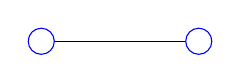
\begin{tikzpicture}
    \node[shape=circle, draw=blue] (A) at (-1,0) {};
    \node[shape=circle, draw=blue] (B) at (1,0) {};

    \path [-] (A) edge (B);
  \end{tikzpicture}
\end{example}

\begin{definition}\cite[Definition 1.1.3]{wemyss2015grouptheory}
  A symmetry of a graph is a bijection \(f : V \to V\) on such that \(f(v_{1})\) and \(f(v_{2})\) are joined by an edge if and only if \(v_{1}\) and \(v_{2}\) are joined by an edge.
\end{definition}

\begin{example}
  Determine all the symmetries of the following graph:

  \begin{centre}
    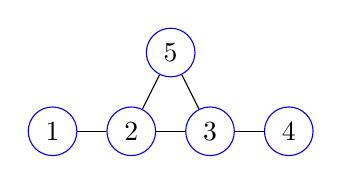
\begin{tikzpicture}
      \node[shape=circle, draw=blue] (1) at (0,0) {1};
      \node[shape=circle, draw=blue] (2) at (1,0) {2};
      \node[shape=circle, draw=blue] (3) at (2,0) {3};
      \node[shape=circle, draw=blue] (4) at (3,0) {4};
      \node[shape=circle, draw=blue] (5) at (1.5,1) {5};

      \path [-]  (1) edge (2);
      \path [-]  (2) edge (3);
      \path [-]  (3) edge (4);
      \path [-]  (2) edge (5);
      \path [-]  (3) edge (5);
    \end{tikzpicture}
  \end{centre}

  Let \(f\) be an arbitrary symmetry.
  %
  By definition, \(f\) must preserve the valency of vertices.
  %
  As vertex 5 is the only vertex of valency 2, we must have that \(f(5) = 5\).
  %
  Since vertices 2 and 3 are the only vertices of valency 3, \(f\) can either fix them, or swap them.
  \begin{enumerate}
  \item
    Suppose they are fixed.
    %
    Then \(f\) fixes both 1 and 4 as \(f(1)\) has valency 1 and must be connected to \(f(2) = 2\), hence \(f(1) = 1\).
    %
    A similar argument applies to vertex 4.
    %
    The completes the case where \(f\) fixes vertex 2 and 3.
  \item
    Suppose they are swapped.
    %
    Then \(f(1) = 4\), as \(f(1)\) must have valency 1 and be connected to \(f(3) = 3\).
    %
    Likewise, \(f(4) = 1\).
  \end{enumerate}

  Hence there are exactly two symmetries.
\end{example}

\begin{note}
  The definition of a symmetry is not dependent on the embedding of the graph in the plane.
  %
  It is easy to visually inspect a graph and gain an intuition about the symmetries, but a formal proof requires one to be more precise.
\end{note}



% *** Groups and examples
\section{Groups and examples}

\begin{definition}\label{def:intro-to-group-theory:group}
  A \indx{group} \(G\) is a set \(G\) equipped with a binary operation \(* : G \times G \to G\), a unary operation \((-)^{-1}: G \to G\), and an identity element \(e \in G\) such that the following properties hold:

  \begin{enumerate}
    \item \(*\) is associative (\((g * h) * j = g * (h * j)\));
    \item \(e * g = g = g * e\), for all \(g \in G\);
    \item \(g * g^{-1} = e = g^{-1} * g\).
  \end{enumerate}

  The \indx{order} of a group \(G\), denotes \(|G|\) is the cardinality of the underlying set.

  The \indx{order} of an element \(g \in G\) is the smallest natural number \(n\) such that \(g^{n} \coloneqq \underbrace{g * g * \ldots * g}_{n} = e\).
\end{definition}


We may sometimes explicitly denote the group and its operation, when it is necessary, by \((G, *)\).

\begin{example}
  The automorphisms of an object (i.e the symmetries of a graph) form a group.
\end{example}


\begin{example}
  The integers \(\Z\) form a group under addition.
\end{example}


\begin{example}\label{ex:group-theory:symmetric-group}
  \(S_{n}\), the \index{symmetric group} on \(n\) elements is the set of permutations of \(\{1, \ldots, n\}\).
  %
  It is a group under composition.


  We typically use cycle notation \((123)(12): S_{3} \to S_{3}\), where \((123)\) means the permutation sending 1 to 2, 2 to 3 and 3 to 1.
  %
  Two bracket cycles next to each other for a permutation by composition.
\end{example}

\begin{example}
  The \(n^{\text{th}}\) \indx{dihedral} group is the group of symmetries of the \(n\)-gon.
  %
  It has \(2n\) elements: \(n\) rotations and \(n\) reflections.

  \begin{centre}
    \begin{tikzpicture}
      \node[shape=circle, draw=blue] (A) at (-1,1) {};
      \node[shape=circle, draw=blue] (B) at (1,1) {};
      \node[shape=circle, draw=blue] (C) at (1,-1) {};
      \node[shape=circle, draw=blue] (D) at (-1,-1) {};

      \node[] (E) at (2,2) {};
      \node[] (F) at (-2,-2) {};
      \node[] (G) at (0,2) {};
      \node[] (H) at (0,-2) {};

      \path [-] (A) edge (B);
      \path [-] (B) edge (C);
      \path [-] (C) edge (D);
      \path [-] (D) edge (A);

      \path [-] (E) edge (F);
      \path [-] (G) edge (H);
    \end{tikzpicture}
  \end{centre}
\end{example}
% TODO add more examples



% *** Subgroups and Lagrange's Theorem
\section{Subgroups and Lagrange's Theorem}

\begin{definition}\label{def:group-theory:subgroup}
  A \indx{subgroup} \(H\) of a group \(G\) is a subset \(H \subset G\) such that it is still a group under the restriction of the structure of \(G\) to \(H\).
  %
  That is, if the following hold:
  \begin{enumerate}
  \item For all \(h, k \in H\), \(hk \in H\);
  \item For all \(h \in H\), \(h^{-1} \in H\).
  \end{enumerate}


  We write \(H \leq G\) to say that \(H\) is a subgroup of \(G\).
\end{definition}


\begin{lemma}[Subgroup criterion]
  \label{lem:group-theory:subgroup-criterion}
  Let \(H \subset G\).
  %
  Then \(H \leq G\) if and only if \(hk^{-1} \in H\) for all \(h,k \in H\).
\end{lemma}


\begin{example}
  The group of rotations of an \(n\)-gon are a subgroup of \(D_{n}\).
\end{example}


\begin{example}
  The \(n\)-th \indx{alternating group}, denoted \(A_{n}\) is the subgroup of \(S_{n}\) consisting of all permutations that can be written as the product of an even number of 2-cycles.
\end{example}

\begin{example}
  Let \(F\) be a field.
  %
  The \indx{general linear group} \(GL(n, F)\) is the set of all invertible \(n \times n\) matrices over \(F\).
  %
  The \indx{special linear group} \(SL(n, F)\) is the set of all \(n \times n\) matrices over \(F\) with determinant \(1\).
  %
  It is a subgroup of \(GL(n, F)\).
\end{example}

\begin{example}\label{ex:group-theory:centre-subgroup}
  Let \(G\) be a group. The subset \(\{ g \in G \mid gh = hg, \forall h \in G\}\) is called the \indx{centre of \(G\)}, and is a subgroup of \(G\).
\end{example}


An important construct from a subgroup \(H \leq G\) is that of the left and right cosets.

\begin{definition}\label{def:group-theory:coset}
  Let \(H \leq G\), and \(g \in G\).
  %
  The \indx{left coset} of \(H\) determined by \(g\) is the set \(gH \coloneqq \{gh \mid h \in H\}\).
  %
  Similarly, the \indx{right coset} of \(H\) determined by \(G\) is \(Hg\).


  The number of left cosets of a subgroup \(H \leq G\) is called the \indx{index} of \(H\) in \(G\), and is denoted \([G : H]\).
\end{definition}

\begin{example}
  Let \(G\) be a group and let \(g \in G\).
  %
  Then, \(\langle g \rangle \coloneqq \{g^{n} \mid n \in \Z\}\) is a subgroup of \(G\) called the \indx{subgroup generated by \(g\)}.
  %
  If \(G = \langle g \rangle\) for some \(g \in G\), then we say that \(G\) is \indx{cyclic}.
\end{example}

\begin{lemma}
  \label{lem:group-theory:cosets-partition-a-group}
  Let \(H \leq G\) be a subgroup. Then the cosets \(gH\) partition the group \(G\).
\end{lemma}

\begin{proof}
  Suppose that \(g \in aH\) and \(g \in bH\), for some \(a, b \in G\).
  %
  Then some simple algebra shows that \(a \in bH\) and \(b \in aH\), from which we deduce that \(a = b h_{1}\) and \(b = a h_{2}\) for some \(h_{1}, h_{2} \in H\).
  %
  Then any \(ah \in aH\) is equal to \(bh_{1}h \in bH\), so \(aH \subset bH\).
  %
  Similarly, we can show that \(bH \subset aH\), and so \(aH = bH\).
  %
  Therefore \(aH = bH\) or \(aH \cap bH = \emptyset\).
  %
  It is also clear that every \(g \in G\) is in \(gH\), and so cosets partition \(G\).
\end{proof}

\begin{lemma}
  If \(G\) is a cyclic group, then either \(G \iso C_{n}\) for some \(n \in \N\) or \(G \iso (\Z, +)\).
\end{lemma}

We reach the titular theorem of this section.

\begin{theorem}[Lagrange's Theorem]\label{thm:group-theory:Lagranges-theorem}
  Let \(H\) be a subgroup of a finite group \(G\). Then
  \[|G| = [G : H]|H|.\]
\end{theorem}

\begin{proof}
  This follows from Lemma~\ref{lem:group-theory:cosets-partition-a-group}, along with the fact that each coset has the same size.

  It is also clear that the function \(ah_{1} \mapsto bh_{1}\)  from \(aH \to bH\) is a bijection, and so any two left cosets of H have the same cardinality.

  This completes the proof of Lagrange's Theorem.
\end{proof}



\begin{corollary}
\label{cor:group-theory:order-divides-group}
  Suppose \(G\) is a finite group and \(g \in G\).
  %
  Then, \(o(g) \mid \left|G\right|\).
\end{corollary}

\begin{proof}
  The subgroup \(\langle g \rangle \leq G\) has order \(o(g)\), and so by Lagrange's theorem, \(o(g)\) must divide \(|G|\).
\end{proof}

\begin{corollary}
\label{cor:group-theory:g-to-power-of-group-order-is-e}
  Suppose \(G\) is a finite group.
  %
  For all \(g \in G\), \(g^{\abs{G}} = e\).
\end{corollary}

\begin{proof}
  By Corollary~\ref{cor:group-theory:order-divides-group}, \(|G| = k \times o(g)\), for a fixed \(g \in G\).
  %
  Then, \(g^{\abs{G}} = g^{k \times o(g)} = e^{k} = e\).
\end{proof}

\begin{corollary}
  Let \(G\) be a finite group.
  %
  If \(\abs{G}\) is prime, then \(G\) is cyclic.
\end{corollary}

\begin{proof}
  If \(\abs{G}\) is prime, the only subgroups are \(\{e\}\) and \(G\).
  %
  Since \(\langle g \rangle \leq G\) is non-trivial for non-identity elements \(g \in G\), it must be the whole group.
  %
  Therefore, \(G\) is equal to a cyclic subgroup and is cyclic itself.
\end{proof}


Lagrange's Theorem can be used to prove Fermat's second most famous theorem.

\begin{theorem}
 \label{thm:group-theory:fermats-little-theorem}
 If \(p\) is a prime and \(a \in \Z\), then
 \[a^{p} \equiv a \mod p.\]
\end{theorem}

\begin{proof}
  This holds trivially for \(a = 0\), so assume \(a \not\equiv 0 mod p\).
  %
  Then, \(g\) is in the multiplicative group of units \(\Z^{*}_{p}\), which has order \(p-1\). By Corollary~\ref{cor:group-theory:g-to-power-of-group-order-is-e}, \(a^{p-1} \equiv 1 \mod p\), and so \(a^{p} \equiv a \mod p\).
\end{proof}

Wilson's Theorem also follows as an application of Lagrange's Theorem.

\begin{theorem}[Wilson's Theorem]
  \label{thm:group-theory:wilsons-theorem}
  If \(p\) is a prime number then the following hold:
  \begin{enumerate}
  \item
    In \(\Z^{*}_{p}\), only \(1\) and \(p-1\) are their own inverses.
  \item
    \((p - 1)! \equiv -1 \mod p\).
  \end{enumerate}
\end{theorem}

\begin{proof}
  We prove both parts.
  \begin{enumerate}
  \item
    Clearly, 1 and \(p-1\) are their own inverses.
    %
    Take \(1 < a < p -1\).
    %
    Neither \(a-1\) nor \(a+1\) are multiples of \(p\) and as \(p\) is prime, \((a-1)(a+1) = a^{2} -1\) is not a multiple of \(p\).
    %
    Therefore, \(a^{2}-1 \not\equiv 0 \mod p\), and so \(a^{2} \not\equiv 1 \mod p\) proving that \(a\) is not its own inverse.

  \item
    This follows by a simple counting argument.
    %
    Every element \(a \in \{2, \ldots, p-2\}\) can be paired up with its inverse, which is also in that range.
    %
    Therefore, the product \((p-1)! \equiv p-1 \equiv -1 \mod p\).
  \end{enumerate}
\end{proof}



% *** Group homomorphisms
\section{Group homomorphisms}
\label{sec:group-theory:group-homomorphisms}

We now turn to the morphisms between groups.

\begin{definition}
  \label{def:group-theory:group-homomorphism}
  Let \(G, H\) be groups.
  %
  A function \(\phi : G \to H\) such that \(\phi(ab) = \phi(a) \phi(b)\), for all \(a, b \in G\) is a \indx{group homomorphism}.
\end{definition}

\begin{lemma}
  Let \(\phi : G \to H\) be a group homomorphism.
  %
  Then the following hold:
  \begin{enumerate}
  \item
    \(\phi(e) = e\) and \(\phi(g^{-1}) = \phi(g) ^{-1}\).
  \item
    If \(\phi\) is injective, then \(o(g) = o\left(\phi(g)\right)\).
  \end{enumerate}
\end{lemma}

\begin{proof}
  \begin{enumerate}
  \item
    We have the following equalities hold:
    \begin{align*}
      \phi(e) &= \phi(ee) \\
              &= \phi(e) \phi(e).
    \end{align*}
    %
    Therefore, we can apply \(\phi(e)^{-1}\) to both sides of the equation and cancel to get \(\phi(e) = e\).
    %
    Recalling that inverses are unique, \(\phi(g)\phi(g^{-1}) = \phi(gg^{-1}) = \phi(e) = e\).
    %
    Applying the similar proof by multiplying \(\phi(g)\) on the left, we deduce that \(\phi(g^{-1}) - \phi(g)^{-1}\).

  \item
    Suppose that \(o(\phi(g)) = n\).
    %
    Then, \(e = \phi(e) = \phi(g)^{n} = \phi(g^{n})\), and so by injectivity of \(\phi\), \(e = g^{n}\).
    %
    Suppose there exists \(0 < k < n\) such that \(g^{k} = e\). Then, \(e = \phi(e) = \phi(g^{k}) = \phi(g)^{k}\), which contradicts \(n\) being the order of \(o(\phi(g))\). Hence \(n\) is the order of \(g\).

  \end{enumerate}
\end{proof}

\begin{example}
  Let \(C_{n}\) be the \indx{cyclic group of order \(n\)}, which is defined as the set of rotations of the equilateral \(n\)-gon.
  %
  If \(g\) is a rotation by \(2 \pi /n \) radians, then \(C_{n} \coloneqq \langle g \rangle\).
  %
  The function
  \begin{align*}
    \phi : \Z &\to C_{n} \\
    a &\mapsto g^{a}
  \end{align*}
  is a group homomorphism.
\end{example}


\begin{definition}
  \label{def:group-theory:group-isomorphism}
  Let \(G, H\) be groups and \(\psi : G \to H\) a group homomorphism.
  %
  We say that \(\phi\) is a \indx{group isomorphism} if there is a group homomorphism \(\psi\) such that \(phi\) and \(\psi\) are inverse functions.

  If there exists an isomorphism \(\psi : G \to H\), we say \(G\) and \(H\) are \indx{isomorphic as groups}, and write \(G \iso H\).
\end{definition}

\begin{lemma}
  \label{lem:group-theory:groups-of-order-p-are-isomorphic}
  If \(p\) is a prime number, then all groups of order \(p\) are isomorphic.
\end{lemma}

\begin{proof}
  Let \(G, H\) be groups of order \(p\).
  %
  Then, every non-identity element has order \(p\), since by Lagrange's Theorem every non-trivial subgroup is equal to the whole group.
  %
  Choose a non-identity element \(g \in G\) and \(h \in H\).
  %
  The function mapping \(g^{n} \mapsto h^{n}\) is well defined and is a bijective group homomorphism.
  %
  Hence, \(G \iso H\).
\end{proof}

\begin{lemma}
  All cyclic groups of order \(n\) are isomorphic.
\end{lemma}

\begin{proof}
  This is the same proof as Lemma~\ref{lem:group-theory:groups-of-order-p-are-isomorphic}.
\end{proof}


Given a group homomorphism, we can always extract a new group from it.

\begin{definition}
  Let \(\phi:G \to H\) be a group homomorphism.
  %
  The \indx{kernel} of \(\phi\) is the subset \(\{g \in G \mid \phi(g_) = e\}\).
\end{definition}

\begin{lemma}
\label{lem:group-theory:kernels-are-subgroups}
  The kernel of a homomorphism \(\phi : G \to H\) (denoted \(\ker(\phi)\)) is a subgroup of \(G\).
\end{lemma}

\begin{proof}
 Clearly, for all \(g, h \in \ker(\phi)\) we have that \(\phi(gh^{-1}) = \phi(g)\phi(h)^{-1} = e\), and as \(e \in \ker(\phi)\), \(\ker (\phi)\) is a subgroup of \(G\).
\end{proof}


\begin{lemma}
  A group homomorphism \(\phi : G \to H\) is injective if and only if \(\ker{\phi} = \{e\}\).
\end{lemma}

\begin{proof}
  Supposing that \(\phi\) is injective, as \(\phi(e) = e\), all elements of the kernel (which are of the form \(\phi(g)\)) must be equal to \(e\).

  Assuming the kernel is trivial, \(\phi(g) = \phi(h)\) implies \(\phi(gh^{-1}) = e\), and so \(gh^{-1} = e\).
  %
  Therefore, \(g = h\) and \(\phi\) is injective.
\end{proof}

\begin{definition}
  Let \(\phi : G \to H\) be a group homomorphism.
  %
  The \indx{image} of \(\phi\) is defined as \(\{\phi(g) \in H \mid g \in G\}\), and is denoted \(\Im \phi\).
\end{definition}

\begin{lemma}
  Let \(\phi : G \to H\) be a group homomorphism.
  %
  The \(\Im \phi\) is a subgroup of \(H\).
\end{lemma}

\begin{proof}
  Let \(g, h \in \Im \phi\).
  %
  Then \(gh^{-1} = \phi(a)\phi(b)^{-1} = \phi(ab^{-1})\), for some \(a,b \in G\).
  %
  As \(e = \phi(e) \in \Im \phi\), \(\Im \phi\) is non-empty and by the Subgroup Criterion, \(\Im \phi\) is a subgroup of \(H\).
\end{proof}

\begin{definition}
  \label{def:group-theory:automorphism-group}
  Let \(G\) be a group.
  %
  The set of all isomorphisms \(\phi : G \to G\) forms a group with composition and inverses, and is called the \indx{automorphisms group} of \(G\), denoted \(\Aut (G)\).
\end{definition}

\begin{example}
  For prime \(p\), \(\Aut(C_{p}) \iso \Z^{*}_{p} \iso C_{p-1}\).
\end{example}

\begin{definition}
  Let \(G, H\) be groups.
  %
  The \indx{product group} \(G \times H\) is the group of pairs of elements \(g \in G, h \in H\), with group operations defined pointwise.
\end{definition}

\begin{example}
  For coprime \(m, n\), \(C_{m} \times C_{n} \iso C_{mn}\).
  %
  The element \((1,1) \in C_{m} \times C_{n}\) must have order \(mn\), hence \(\langle (1,1)\rangle= \C_{m} \times C_{n}\) is isomorphic to the cyclic group of order \(mn\).
  %
  If there is a \(1 < k < mn\) such that \((1,1)^{k} = (0,0)\), then \(k\) would need to share a factor of both \(m\) and \(n\), which would contradict coprimality.
\end{example}



% *** Isomorphism theorems
\section{Isomorphism theorems}
\label{sec:group-theory:isomorphism-theorems}

Arguably, the most important type of subgroup is the normal subgroup.

\begin{definition}
  A subgroup \(H \leq G\) is said to be \indx{normal} if \(gH = Hg\) for all \(g \in G\).
  %
  We denote this by \(H \triangleleft G\).
\end{definition}

\begin{lemma}
 \label{lem:group-theory:normal-subgroup-criterion}
  A subgroup \(H \leq G\) is normal if and only if for all \(g \in G\), \(h \in H\), we have \(g^{-1}hg \in H\).
\end{lemma}

\begin{proof}
  Suppose that \(H \triangleleft G\) is a normal subgroup and let \(g \in G\) and \(h \in H\).
  %
  Since \(gH = Hg\) if and only if \(H = g^{-1}Hg\) and \(g^{-1}hg \in  g^{-1}Hg\), we have \(g^{-1}Hg \in H\), as required.

  Now, assuming that \(g^{-1}hg \in H\) for all \(g \in G\), \(h \in H\), we have that \(g^{-1} H g \subset H\). However, as \(H = g^{-1}gHg^{-1}g \subset g^{-1}Hg\), we must have that \(H = g^{-1}Hg\) and so \(gH = Hg\), proving that \(H\) is normal in \(G\).
\end{proof}

\begin{example}[Examples of normal subgroups]\label{ex:group-theory:normal-subgroups}
  \begin{enumerate}
  \item For any group \(G\), the centre \(Z(G)\) is normal, since every \(g \in G\) commutes with all elements in \(Z(G)\).
  \item Any subgroup of an abelian group is normal.
  \end{enumerate}
\end{example}

As left and right cosets are the same for a normal subgroup \(N \triangleleft G\), we typically just refer to them as ``cosets'', choosing to work with left cosets if necessary.

\begin{definition}
  \label{def:group-theory:quotient-group}
  Let \(N \triangleleft G\) be a normal subgroup. The set of cosets is denoted \(G / N\) and has a canonical group structure associated with it, defined by \(gN * hN = (gh)N\) and \((gN)^{-1} \coloneqq (g^{-1})N\). Groups of this form are called \indx{quotient groups}.
\end{definition}

This group structure is well defined for normal subgroups, but not always for arbitrary subgroups.
%
To show that it is well defined, suppose \(g_{1}N = g_{2}N\) and \(h_{1}N = h_{2}N\).
%
We need to show that \(g_{1}h_{1}N = h_{1}h_{2}N\).
%
This follows by normality of \(N\):

\[g_{1}h_{1} N = g_{1} h_{2}N =g_{1}Nh_{2} = g_{2}Nh_{2} = g_{2}h_{2}N.\]

Inverses is well defined, also by normality, for if \(g_{1}N = g_{2}N\), then we have the following equations:
\[(g_{1}N)^{-1}g^{-1}_{2} = g_{1}^{-1}Ng^{-1}_{2} = g_{1}^{-1}g_{2}N = g^{-1}_{1}g_{1}N = N.\]

Hence, \((g^{-1}_{1}N) = (g_{1}N)^{-1} = Ng_{2} = (g^{-1}_{2}N)\), as required.


\begin{theorem}
  Let \(G\) be a group and \(N \leq G\) a subgroup.
  %
  Then, \(N \triangleleft G\) if and only if \(N\) is the kernel of some group homomorphism from \(G \to H\).
\end{theorem}

\begin{proof}
  Suppose that \(N \triangleleft G\).
  %
  Then, there is a canonical function \(\phi: G \to G/N\) mapping \(g \mapsto gN\).
  %
  This function is a group homomorphism, as
  \[\phi(gh) = ghN = gN * hN = \phi(g) * \phi(h). \]
  %
  It is clear that the kernel of this morphism is \(N\).

  Now, supposing that \(N = \ker(\phi)\), for some \(\phi : G \to K\), Lemma~\ref{lem:group-theory:kernels-are-subgroups} shows that \(N \leq G\).
  %
  If \(g \in G\) and \(h \in N\), then
  \[\phi(g^{-1}h g) = \phi(g^{-1}) \phi(h) \phi(g) = \phi(g^{-1})\phi(g) = e,\]
  and so \(g^{-1}h g \in N\), which proves that \(N \triangleleft G\) by Lemma~\ref{lem:group-theory:normal-subgroup-criterion}.
\end{proof}



% **** First Isomorphism Theorem
\subsection{First Isomorphism Theorem}\label{sec:group-theory:first-isom-theorem}

Quotient groups have the a universal property.

\begin{theorem}\label{thm:group-theory:universal-property-of-quotient-groups}
  Let \(N \triangleleft G\) be a normal subgroup, and \(f : G \to H\) be a group homomorphism with \(N \subset \ker(f)\).
  %
  Then there is a unique group homomorphism \(\hat f : G/N \to H\) that makes the following diagram commute:
  \begin{center}
    \begin{tikzcd}
      G \arrow[r, "\phi"] \arrow[rd, "f"'] & G/N \arrow[d, "\hat f", dashed] \\
      & H
    \end{tikzcd}
  \end{center}
\end{theorem}

\begin{proof}
  The map \(\hat f: G/N \to H\) is defined by \(gN \mapsto f(g)N\).
  %
  It is a well defined function as if \(g_{1}N = g_{2}N\), \(g_{1}g^{-1}_{2} \in N \subset \ker(f)\), and so \(f(g_{1})=f(g_{2})\) giving the desired result that \(f(g_{1})N = f(g_{2})N\).
  %
  It is a group homomorphism as \(f\) is a group homomorphism.
  %
  If there was another map \(k:G/N \to H\) that made this diagram commute, then \(k(gN) = (k \circ \phi)(g) = f(g)\), and so \(k(gN) = f(g) = \bar f (gN)\), proving that \(k = \bar f\).
\end{proof}

\begin{categorybox}
  This universal property can be seen categorically as saying the map \(\phi\) is a coequaliser in the category of groups of the diagram:

  \begin{centre}
    \begin{tikzcd}
      N \arrow[r, "i", hook, shift left] \arrow[r, "0"', shift right] & G.
    \end{tikzcd}
  \end{centre}

\end{categorybox}

This result essentially gives us the First Isomorphism Theorem for groups.

\begin{theorem}[First Isomorphism Theorem]
  \label{thm:group-theory:first-isomorphism-theorem}
  Let \(\theta : G \to H\) be a group homomorphism.
  %
  Then, \(N \coloneqq \ker\phi\) is a normal subgroup of \(G\), \(\Im \theta\) is a subgroup of \(H\) and there is an isomorphism
  \[\bar \theta : G / N \to \Im \theta.\]

  In particular, if \(\theta\) is surjective, then \(G / \ker(\theta) \iso H\).
\end{theorem}

\begin{proof}
  The map \(\bar \theta\) is given by Theorem~\ref{thm:group-theory:universal-property-of-quotient-groups}.
  %
  It is clear that the image of \(\bar\theta\) is \(\Im \theta\), since \(\theta(g) = \bar \theta(gN)\), and if \(\bar\theta\) is surjective, it witnesses an isomorphism \(G/\ker(\theta) \iso \Im \theta\).
\end{proof}

\begin{example}
  There is a surjective group homomorphism \(\exp : (\C, +) \to (\C^{*}, \times)\).
  %
  The kernel of \(\exp\) is the set \(N = \{2k\pi i \mid k \in \Z\}\), so \(\C^{*} \iso \C/N\).
\end{example}


% **** The Second and Third Isomorphism Theorems and the Correspondence Theorem
\subsection{The Second and Third Isomorphism Theorems and the Correspondence Theorem}\label{sec:second-and-third-isomorphism-theorems-and-correspondence-theorem}

The second and third isomorphism theorems gives us information about relating the subgroups structure of \(G /N\) to the subgroup structure of \(G\).

\begin{proposition}\label{prp:group-theory:preimage-of-subgroups-of-G/N}
  Let \(G\) be a group and let \(N \triangleleft G\).
  %
  Let \(\theta: G \to G/N\) be the canonical morphism from Theorem~\ref{thm:group-theory:universal-property-of-quotient-groups}, and let \(K \leq G / N\).

  \begin{enumerate}
  \item
    \(\theta^{-1}(K) \leq G\), with \(N \subset \theta^{-1}(K)\).
  \item
    \(\theta^{-1}(K) \triangleleft G\) if and only if \(K \triangleleft G/N\).
  \end{enumerate}
\end{proposition}

\begin{proof}
  \begin{enumerate}
  \item
    It's clear that the preimage is a subset of \(G\) that contains \(e\).
    %
    Let \(g, h \in \theta^{-1}(K)\).
    %
    We see that \(\theta(gh^{-1}) = \theta(g)\theta(h)^{-1}\), which is in \(K\) since it is a subgroup.
    %
    Hence by Lemma~\ref{lem:group-theory:subgroup-criterion}, it is a subgroup of \(G\).

    \item
      Supposing that \(\theta^{-1}(K) \triangleleft G\) and let \(gN \in G/N\) and \(kN \in K\).
      %
      We see that \(k \in \theta^{-1}(K)\), and as the preimage is normal in \(G\), \(g^{-1}kg \in \theta^{-1}K\).
      %
      Therefore, \(g^{-1}kgN = (g^{-1}N)*(kN)*(gN) \in K\), and so \(K \triangleleft G/N\).

      Now, assume that \(K \triangleleft G/N\) and let \(g \in G\), \(h \in \theta^{-1}(K)\).
      %
      \(g^{-1}hgN = (g^{-1}N)*(hN)*(gN) \in K\) by normality of \(K\) and \(hN \in K\).
      %
      Therefore, \(\theta^{-1}(K) \triangle G\), as required.
      %
      This completes the proof.

  \end{enumerate}
\end{proof}

\begin{proposition}\label{prp:group-theory:normal-subgroups-pullback}
  Let \(N \triangleleft G\) and \(\theta : G \to G/N\) as above. If \(N \leq H \leq G\), then \(H = \theta^{-1}\theta(H)\).
  %
  That is, all subgroups of \(G\) that contain \(N\) are pulled back from subgroups of \(G/N\).
\end{proposition}

\begin{proof}
  It is clear that, \(H \subset \theta^{-1}\theta (H)\).
  %
  If \(g \in \theta^{-1}\theta(H)\), then \(\theta(g) \in \theta(H)\) and there must exists \(h \in H\) such that \(\theta(g) = \theta(h)\).
  %
  This means that \(\theta(g h^{-1}) = e_{G/N}\) and so \(g h^{-1} \in N \subset H\).
  %
  Therefore, \(g = h(h^{-1}g) \in H\) and so \(H = \theta^{-1}\theta(H)\), as required.
\end{proof}



These two propositions allow us to prove the following:

\begin{theorem}[The Correspondence Theorem]
  \label{thm:group-theory:the-correspondence-theorem}
  Let \(G\) be a group with \(N \triangleleft G\) and \(\theta: G \to G/N\) the canonical morphism.
  %
  The map \(H \mapsto \theta(H)\) is a bijection between subgroups of \(G\) containing \(N\) and subgroups of \(G/N\).
  %
  Under this bijection, normal subgroups match with normal subgroups; further, if \(N \subset A,B\) are subgroups of \(G\), then \(\theta(A) \subset \theta(B)\) if and only if \(A \subseteq B\).
\end{theorem}

\begin{proof}
  Injectivity of the function follows immediately from Proposition~\ref{prp:group-theory:normal-subgroups-pullback}.
  %
  Part 1 of Proposition~\ref{prp:group-theory:preimage-of-subgroups-of-G/N} shows that the function is surjective (since \(\theta\theta^{1}K = K\) and \(N \subset \theta^{-1}(K)\)).
  %
  Part 2 of Proposition~\ref{prp:group-theory:normal-subgroups-pullback} shows us that normal subgroups match up with normal subgroups.
  %
  Now, supposing that \(N \leq A \leq B \leq G\), it is clear that \(A/N \subset B/N\).
  %
  Suppose that \(A/N \subset B/N\) and let \(a \in A\).
  %
  There must be \(b \in B\) such that \(aN = bN\), and so \(ab^{-1} \in N\).
  %
  This means \(a = bn \in B\), for some \(n \in N\).
  %
  Hence, \(a \in B\) and \(A \subseteq B\).
\end{proof}

\begin{example}
  Since \(\Z\) is abelian, all of its subgroups are normal.
  %
  We can determine all of the subgroups of \(\Z/12Z\) by finding all of the subgroups of \(\Z\) that contain \(12\Z\).
  %
  These are \(\Z, 2\Z, 3\Z\) and \(4\Z\).
  %
  Under the correspondence, they give the subgroups \(12\Z\), \(2\Z / 12\Z\), \(3\Z / 12\Z\) and \(4\Z / 12\Z\).
  %
  There is a surjective group homomorphism \(2\Z / 12\Z \to \Z/6\Z\) mapping \(2n(12\Z) \mapsto n(6Z)\).
  %
  It is well defined as if \(2m(12\Z) = 2n(12\Z)\) then \(m(6\Z) = n(6\Z)\) and it is easy to show that it is a group homomorphism.
  %
  Theorem~\ref{thm:group-theory:first-isomorphism-theorem} gives us that \((2\Z) / (12\Z) \iso \Z/6\Z\), and likewise, \((m\Z) / (n\Z) \iso \Z/(\frac n m)\Z\).
\end{example}

The Third Isomorphism Theorem tells us how to work with groups of the form \((G/N)/(H/N)\).

\begin{theorem}[The Third Isomorphism Theorem]
  \label{thm:group-theory:the-third-isomorphism-theorem}
  If \(N \leq H \leq G\), with \(N, H \triangleleft G\), then
  \[(G/N)/(H/N) \iso G/H.\]
\end{theorem}

\begin{proof}
  We have the following diagram:
  \begin{center}
    \begin{tikzcd}
      G \arrow[r, "\can_N"] \arrow[rd, "\can_H"'] & G/N \arrow[d, "\pi", dashed] \\
      & G/H
    \end{tikzcd}
  \end{center}

  Since \(N \subset H\), \(N \leq \ker(\can_{H})\) and Theorem~\ref{thm:group-theory:universal-property-of-quotient-groups} gives us the existence of \(\pi\).
  %
  Since \(\can_{H}\) is surjective, \(\pi\) is also surjective.
  %
  We now show that \(\ker(\pi) = H/N\), and use Theorem~\ref{thm:group-theory:universal-property-of-quotient-groups} to deduce the result.
  %
  Let \(hN \in H/N\).
  %
  Then, \(\pi(hN) = \can_{H}(h) = e\), so \(hN \in \ker(\pi)\).
  %
  Let \(gN \in \ker(\pi)\).
  %
  Then, \(e = \pi(gN) = \can_{H}(g)\), so \(g \in H\) which means that \(gN \in H/N\).
  %
  This shows that \(H/N = \ker(\pi)\) and so \((G/N) / (H/N) \iso G/H\).
\end{proof}

What can we say about subgroups of \(H \leq G\) that don't contain the normal subgroup \(N\)?

\begin{theorem}[The Second Isomorphism Theorem]
 \label{thm:group-theory:second-isomorphism-theorem}
 Let \(N \triangleleft G\) be a normal subgroup of a group \(G\) and  \(H \leq G\) a subgroup of \(G\).
 %
 Then, the following hold:
 \begin{enumerate}
 \item
   \(HN \coloneqq \{hn \mid h \in H, n \in N\}\) is a subgroup of \(G\);
 \item
   \(N \triangleleft HN\);
 \item
   \(H \cap N \triangleleft H\);
 \item
   There exists an isomorphism
   \[HN/N \iso H/(H\cap N).\]
 \end{enumerate}
\end{theorem}

\begin{proof}
  \begin{enumerate}
  \item
    It is clear that \(e \in HN\).
    %
    Let \(h_{1}, h_{2} \in H\) and \(n_{1}, n_{2} \in N\).
    %
    Then, \(h_{1}n_{1}(h_{2}n_{2})^{-1} = h_{1}n_{1}n_{2}^{-1}h_{2}^{-1}\).
    %
    Since, \(N \triangleleft G\), \(n_{1}n_{2}^{-1}h_{2}^{-1} \in Nh_{2}^{-1} = h_{2}^{-1}N\), \(n_{1}n_{2}^{-1}h_{2}^{-1} = h_{2}^{-1}n_{3}\), for some \(n_{3} \in N\), we can deduce the following:

    \[(h_{1}n_{1})(h_{2}n_{2})^{-1} = h_{1}n_{1}h_{2}^{-1}h_{2}^{-1} = h_{1}h_{2}^{-1}n_{3} \in HN,\]
    and so \(HN \leq G\).

    \item
      \(N\) is normal in \(HN\) since all elements of \(HN\) are also elements of \(G\).

    \item
      Let \(a \in H \cap N\).
      %
      Then, for all \(h \in H\), \(hah^{-1} \in H\).
      %
      Since \(N \triangleleft G\) and \(H \subset G\), \(hah^{-1} \in N\), and so \(hah^{-1} \in H \cap N\), which proves \(H\cap N \triangleleft H\).
    \item
     By the Correspondence Theorem (Theorem~\ref{thm:group-theory:the-correspondence-theorem}) and \(N \subset HN\), we have a group homomorphism \(\can_{N}|_{H}: H \to H/N\).
     %
     The kernel of this map is the set \(\{n \in H \mid n \in N\} = N \cap H\), and the image is \(HN/N\) (follows from \(hN = heN \in HN/N\) and \(hnN = hN\)).
     %
     Hence, the First Isomorphism Theorem (Theorem~\ref{thm:group-theory:first-isomorphism-theorem}) gives an isomorphism
     \[H/(H\cap N) \iso HN/N.\]
  \end{enumerate}
\end{proof}

\begin{corollary}
  Let \(a,b \in \Z\).
  %
  Then, \(ab = \gcd(a,b)\lcm(a,b)\).
\end{corollary}

\begin{proof}
  We take the function \(\can_{b}|_{a\Z} : a\Z \to Z / b\Z\).
  %
  The first isomorphism theorem gives
  \[\can_{b}|_{a\Z}(a\Z) \iso a\Z / (a\Z \cap b\Z) \iso a\Z / \lcm(a,b)\Z.\]

  Applying the Second Isomorphism Theorem (Theorem~\ref{thm:group-theory:second-isomorphism-theorem}) to the middle term in the isomorphism chain, we get that
  \[a\Z / a\Z \cap b\Z \iso a\Z b\Z / a\Z \iso (a\Z + b\Z)\Z / b\Z \iso \gcd(a,b) \Z / b\Z.\]
  This gives an isomorphism
  \[a\Z/ \lcm(a,b)\Z \iso \gcd(a,b)\Z/ b\Z.\]

  The left hand side has cardinality \(\lcm(a,b)/a\), while the right hand side's cardinality is \(b/\gcd(a,b)\).
  %
  This means \(ab = \gcd(a,b)\lcm(a,b)\), as required.


\end{proof}



% *** Group presentations
\section{Group presentations}
\label{sec:group-theory:group-presentations}

Every group has a \textit{presentation} which describes it wholly.
%
It is formed by taking a free group and quotienting selected elements to the identity.

\begin{definition}\label{def:group-theory:free-group}
  The \indx{free group} on generators \(x_{1}, x_{2}, \ldots, x_{n}\) is the group whose elements are words in the symbols \(x_{1}, \ldots, x_{m},x^{-1}, \ldots, x^{-1}_{m}\), subject to the group axioms and all logical consequences.
  %
  The group operation is concatenation.
  %
  It is written as \(\langle x_{1}, \ldots, x_{m} \rangle\).
\end{definition}

\begin{definition}
 \label{def:group-theory:generated-by-subject-to-relations}
 Let \(r_{1}, \ldots, r_{n} \in \langle x_{1}, \ldots, x_{2} \rangle\).
 %
 The group \indx{generated} by \(x_{1}, \ldots, x_{m}\) subject to the relations \(r_{1}, \ldots, r_{n}\) is the group with generators \(x_{1}, \ldots, x_{m}\), subject to the group axioms, the rules \(r_{1} = r_{2}= \ldots = r_{n} = e\) and all logical consequences.
 %
 We write this group \(\langle x_{1}, \ldots, x_{m} \mid r_{1}, \ldots, r_{n} \rangle\) and call this a presentation of the group.
\end{definition}

\begin{example}
  Let \(D = \langle x \mid x^{3} = x^{2} \rangle\).
  %
  This group must then satisfy \(x=e\) and so this is a presentation the free group.
\end{example}

\begin{theorem}
  \label{thm:group-theory:universal-property-of-free-groups}
  Let \(G\) be a group and \(S\) an arbitrary set.
  %
  There is a bijection between the sets of group homomorphisms \(\langle S \rangle \to G\) and functions \(G \to S\).
\end{theorem}



\section{Sylow theory}
The Sylow Theorems act as a close converse to Lagrange's theorem. The converse to Lagrange's theorem does not hold in general.

\begin{example}
  The alternating group \(A_{4}\) has order \(12\), but has no subgroup of order 6.
\end{example}

The best ``partial'' converse is we have is Cauchy's Theorem:

\begin{theorem}[Cauchy's Theorem]\label{thm:group-theory:cauchys-theorem}
  If \(p\) is a prime that divides the order of \(G\), then \(G\) has a subgroup of order \(p\).
\end{theorem}

We need to introduce some tools before we can prove this result.

\subsection{Group actions}

\begin{definition}\label{def:group-theory:group-action}
  Let \(G\) be a group and \(X\) a set. A (left) \indx{\(G\)-action} (or \indx{\(G\)-set}) on \(X\) is a function

  \[\_ \cdot \_ :  G \times X \to X,\]

  such that the following hold:

  \begin{enumerate}
    \item The identity acts trivially: \(e \cdot x = x\), for all \(x \in X\);
    \item Actions are associative: \(g \cdot (h \cdot x) = (gh \cdot x)\).
  \end{enumerate}

  A morphism between two group actions on sets \(X\) and \(Y\) is a function \(f: X \to Y\) such that \(f(g\cdot x) = g \cdot (f(x))\).
\end{definition}

\begin{categorybox}
  A left group action is equivalently a functor \(G \to \Set\). The functor category \([G, \Set]\) is isomorphic to the category of \(G\)-sets.
\end{categorybox}

Any \(G\)-set gives rise to two important constructions.

\begin{definition}\label{def:group-theory:orbit}
  The \indx{orbit} of a group action is a subset of \(X\) defined as:
  \[G \cdot x \coloneqq \{g \cdot x \mid g \in G\}.\]
\end{definition}

\begin{definition}\label{def:group-theory:stabilizer}
  The \indx{stabilizer} of \(x \in X\) under a group action is the subgroup of \(G\)

  \[\Stab_{G}(x) \coloneqq \{ g \in G \mid g \cdot x = x \}.\]
\end{definition}

\begin{lemma}\label{lem:group-theory:stabilizer-is-subgroup}
  Let \(G\) be a group that acts on a set \(X\). Then, for all \(x \in X\), the stabilizer of the group action is a subgroup of \(G\).
\end{lemma}

\begin{proof}
  Clearly \(e \in \Stab_{G}(x)\). If \(g, h \in \Stab_{G}(x)\), then
  \begin{align*}
    gh^{-1} \cdot x = gh^{-1} \cdot (h \cdot x) = g \cdot x = x.
  \end{align*}

  Therefore, \(gh^{-1} \in \Stab_{G}(x)\) and it is a subgroup of \(G\).
\end{proof}

\begin{example}
  Let \(k\) be a field and let \(n\) be a positive integer. Defining \(G = \GL_{n}(k)\) and \(X = k^{n}\), \(G\) acts on \(X\) by matrix multiplication.
\end{example}

\begin{example}
  Let \(n\) be a positive integer and let \(G = \mathbb S_{n}\), the \(n\)th symmetric group. Let \(X = \{1, \ldots, n\}\). Then \(G\) acts on \(X\) by \(\sigma \cdot i = \sigma(i)\).
\end{example}


\begin{lemma}\label{lem:group-theory:orbits-partition}
  Let \(G\) act on \(X\). Then,
  \begin{enumerate}
    \item The action induces an equivalence relation \(\sim\) on \(X\) defined by: \(x \sim y\) if and only if there exists \(g \in G\) with \(g \cdot x = y\);
    \item The equivalence classes of this relation are the orbits.
    \item The distinct orbits in \(X\) form a partition of \(X\).
  \end{enumerate}
\end{lemma}

\begin{proof}
  It is routine to check that that \(\sim\) is an equivalence relation and that the orbits are the equivalence classes.
\end{proof}

The fundamental theorem about group actions is the following:

\begin{theorem}[Orbit-Stabilizer Theorem]\label{thm:group-theory:orbit-stabilizer}
  Let \(G\) be a finite group acting on a set \(X\) and let \(x \in X\). Then
  \[|G| = |\Stab_{G}(x)| |G \cdot x|.\]
\end{theorem}

\begin{proof}
  This follows from~\nameref{thm:group-theory:Lagranges-theorem}. By Lemma~\ref{lem:group-theory:stabilizer-is-subgroup}, we just need to show that each of the stabilizer's cosets correspond to a unique element of \(G \cdot x\), and visa versa. The maps we construct are \(g \cdot x \mapsto g\Stab_{G}(x)\) and \(g\Stab_{G}(x) \mapsto g\cdot x\). These maps are well defined and inverse to each other, so there is a bijection between the cosets of the stabilizer and \(G \cdot x\). Hence, \(|G| = |\Stab_{G}(x)| |G \cdot x|\).
\end{proof}

We have enough to prove~\nameref{thm:group-theory:cauchys-theorem}.

% TODO Add cyclic group example, with proof that it has no non-trivial subgroups.
\begin{proof}
  \textbf{Proof of~\nameref{thm:group-theory:cauchys-theorem},Theorem~\ref{thm:group-theory:cauchys-theorem}}.

  Let \(G\) be a group with order \(n\), and let \(p\) be a prime number that divides \(n\). Our goal is to show that \(G\) contains an element of order \(p\), which generates a subgroup of order \(p\) in \(G\). Define the set \(X \coloneqq \{(g_{0}, \ldots, g_{n-1}) \mid \prod_{i=0}^{n-1}g_{i} = e\}\). The cyclic group of order \(p\), \(C_{p}\), acts on this group by \(m \cdot (g_{i}) \coloneqq (g_{i + m \mod n})\). Our goal is to show that there must exist a non-identity element which is fixed by this group action.

  By a simple counting argument, we see that \(|X| = |G|^{p-1}\), which is a multiple of \(p\). By Lemma~\ref{lem:group-theory:orbits-partition}, the orbits must partition \(X\), and by The~\nameref{thm:group-theory:orbit-stabilizer}, each orbit must have size \(1\) or \(p\). Choosing a representative for each orbit \(x_{0}, \ldots x_{m-1}\), we have that
  \[|X| = pk = \sum_{i=0}^{m-1} C_{p} \cdot x_{i}.\]
  One of these orbits is a singleton containing the element \((e, \ldots, e)\), so we can write

  \[pk = 1 + \sum_{x_{i} \neq e} C_{p} \cdot x_{i}.\]

  Since the left hand side is a multiple of \(p\), the right hand side must be also. As \(1\) is not a multiple of \(p\), there must exist \(p-1\) representatives that have orbits of size \(1\). Denote one such element by \(\overline x\). We must also have that \(|\Stab_{C_{p}}(\overline x)| = p\), and so \(\overline x = (g \ldots, g)\) for some non-identity element \(g \in G\). Therefore, \(\prod_{i=0}^{p-1}g = e\), and so \(o(g) \leq p\). If the order of \(g\) was less than \(p\), then \(p\) would need to be a multiple of the order. As \(p\) is prime, this is not the case, and so \(o(g) = p\).
\end{proof}

\begin{example}
  Any group \(G\) can act on its underlying set in two different ways. The first is by multiplication, with \(g \dot h \coloneqq gh\), and the second is by conjugation: \(g \cdot h \coloneqq ghg^{-1}\).
\end{example}

\begin{definition}\label{def:group-theory:centralizer}
  Let \(G\) be a group and let \(a \in G\). The \indx{centralizer} \(C_{G}(a)\) is the Stabilizer \(\Stab_{}(a)\) where \(G\) acts on itself by conjugation. It is precisely the set of elements in \(G\) that commute with \(a\): \(\{g \in G \mid ga = ag\}\).
\end{definition}

\begin{definition}\label{def:group-theory:conjugacy-class}
  Let \(G\) be a group and let \(a \in G\). The \indx{conjugacy class of \(a\)} is the orbit of \(a\) where \(G\) acts on itself by conjugation. We denote it by \(\Cl(a) \coloneqq \{gag^{-1} \mid g \in G\}\).
\end{definition}

\begin{corollary}\label{cor:group-theory:centralizer-conjugacy-classes-divide-G}
  Let \(G\) be a finite group. For any \(a \in G\), we have
  \[|G| = |C_{G}(a)| |\Cl(a)|,\]
  and this both \(|C_{G}(a)|\) and \(|\Cl(a)|\) divide \(|G|\).
\end{corollary}

\begin{proof}
  Immediate from the \nameref{thm:group-theory:orbit-stabilizer}.
\end{proof}

\begin{corollary}[Class Equation]\label{cor:group-theory:class-equation}
  Let \(G\) be a finite group. Then, there exists elements \(a_{1}, \ldots, a_{n} \in G\) such that
  \[|G| = \sum_{i=1}^{n} |\Cl(a_{i})|.\]
\end{corollary}

\begin{proof}
  By Lemma~\ref{lem:group-theory:orbits-partition}, the orbits of the conjugacy group action partition \(G\). These orbits are the conjugacy classes, hence we get the above equation.
\end{proof}


\begin{definition}
  Let \(p\) be a prime number. A \indx{\(p\)-group} is a group \(G\) such that each element has order a power of \(p\). If \(|G|\) is finite, then \(G\) is a \(p\)-group if and only if \(|G|\) is a power of \(p\), by~\nameref{thm:group-theory:cauchys-theorem}.
\end{definition}


\begin{theorem}\label{thm:group-theory:p-group-non-trivial-centre}
  Let \(G\) be a non-trivial finite \(p\)-group. Then the centre \(Z(G) \neq \{e\}\).
\end{theorem}

\begin{proof}
  Choose \(a_{1}, \ldots, a_{n} \in G\) such that \(|G| = \sum_{i=1}^{n} |\Cl(a_{i})|\). By Corollary~\ref{cor:group-theory:centralizer-conjugacy-classes-divide-G}, each term in the sum divides \(|G|\), and so for each \(a_{i}\), there exists \(r_{i}\) such that \(|\Cl(a_{i})| = p^{r_{i}}\).

  Noticing that \(a \in Z(G)\) if and only if \(\Cl(a) = {a}\), we can split the sum from the class equation up as follows:
  \[ p^{n} = |G| = \sum_{i=1}^{n} |\Cl(a_{i})| = \sum_{a_{i} \in Z(G)} |\Cl(a_{i})|+ \sum_{a_i \not\in Z(G)} |\Cl(a_{i})|= |Z(G)| + \sum_{a_i \not\in Z(G)}|\Cl(a_{i})|.\]

  As \(|\Cl(a)| = 1\) if and only if \(a \in Z(G)\), each \(\Cl(a_{i})|\) must be a power of \(p\). Since \(p | p^{k}\), we must have \(p | |Z(G)|\) and so \(Z(G)\) is non-trivial.
\end{proof}

\begin{lemma}\label{lem:group-theory:cyclic-centre-implies-abelian}
  If \(G\) is a group with \(G / Z(G)\) cyclic, then \(G\) is abelian.
\end{lemma}

\begin{proof}
  As \(G / Z(G)\) is cyclic, there is some \(h \in G\) such that \(hZ(G)\) generates \(G / Z(G)\). Then, since the cosets partition \(G\), every element \(g \in G\) is equal to \(h^{n}k\), for some \(k \in Z(G)\). The product \(gg'\) is then equal to \(h^{n}kh^{m}k'\) for some \(k, k' \in Z(G)\). Each term in this product commutes with the other terms, since we can swap powers of \(h\) and the centre of a group is exactly the elements that commute with every other element. Hence, \(gg' = h^{n}kh^{m}k' = h^{m}k'h^{n}k = g'g\), and \(G\) is abelian.
\end{proof}

\begin{corollary}
  If \(G\) is a group with \(|G| = p^{2}\), then \(G\) is abelian.
\end{corollary}

\begin{proof}
  By Theorem~\ref{thm:group-theory:p-group-non-trivial-centre}, \(G\) has a non-trivial centre, and so \(|Z(G)|\) is equal to \(p\) or \(p^{2}\). If it equals \(p^{2}\), then \(G\) is abelian, so assume the order of the centre is \(p\). Since \(Z(G)\) is normal in \(G\), we can quotient by it and get that \(G/Z(G)\) has order \(p\) and is therefore cyclic. By Lemma~\ref{lem:group-theory:cyclic-centre-implies-abelian}, \(G\) must be abelian.
\end{proof}


\subsection{The Sylow Theorems}

\begin{definition}\label{def:group-theory:sylow-subgroup}
  Let \(G\) be a finite group and let \(p\) be a prime number. A subgroup \(H \leq G\) is a \indx{\(p\)-subgroup} of \(G\) if it is a \(p\)-group. We say it is a \indx{Sylow \(p\)-subgroup} of \(G\) if its order is the highest power of \(p\) that divides the order of \(G\). We say that \(H\) is a \indx{Sylow subgroup} of \(G\) if its is a Sylow \(p\)-subgroup for some prime \(p\).
\end{definition}

If \(p\) does not divide \(|G|\), then the trivial subgroup is the unique Sylow \(p\)-subgroup of \(G\). When we want to exclude this case, we refer to \indx{non-trivial Sylow \(p\)-subgroups}.

\begin{definition}
  For any group \(G\), let \(n_{p}\) be the number of distinct Sylow \(p\)-subgroups of \(G\).
\end{definition}

It's not obvious that non-trivial Sylow \(p\)-subgroups always exist. The first Sylow Theorem guarantees that they do. The second Sylow Theorem says that for a given \(p\) all Sylow \(p\)-subgroups of \(G\) are conjugate, and the third gives information about the number of Sylow \(p\)-subgroups of \(G\).

\begin{theorem}[Sylow 1]\label{thm:group-theory:Sylow-1}
  Let \(|G| = n\) and \(p\) be a prime that divides \(n\). Write \(n = p^{m}r\), with \(p \not| r\). Then, there exists a subgroup of order \(p^{m}\); that is, there is exists a Sylow \(p\)-subgroup.
\end{theorem}

\begin{proof}
  Define a set \(X \coloneqq \{ A \subset G \mid |A| = p^{m}\}\). This is a set of \textit{subsets} of \(G\). There is a group action we can put on \(X\), namely \(g \cdot A \coloneqq gA\). To prove the First Sylow Theorem, we show that this group action has an orbit whose size is not divisible by \(p\). From this, we can then construct a subgroup of \(G\) with order \(p^{m}\).

  Since \(X\) is formed from all subsets of size \(p^{m}\) from a set of size \(p^{m} r\), \(|X| = {p^{m}r \choose p^{m}}\). We can write

  \[{p^{m}r \choose p^{m}} = \frac{p^{m}r(p^{m}r-1)(p^{m}r -2) \ldots (p^{m}r - (p^{m}-1))}{p^{m}(p^{m} - 1)(p^{m} - 2)\ldots(p^{m} - (p^{m} - 1))}.\]

  Looking at the terms \(p^{m}r - s\) and \(p^{m} - s\) for \(1 \leq s \leq p^{m}-1\), we see that the highest power of \(p\) dividing them both is the same - it is the highest power of \(p\) that divides \(s\). We can then pair up terms on the numerator and denominator that are divisible by the same powers of \(p\). This results in the right hand side of the above equation not being divisible by \(p\), and so \(|X|\) isn't either. As \(X\) is a disjoint union of orbits, there must be at least one orbit whose cardinality isn't divisible by \(p\)\footnote{If this were false, \(|X|\) is equal to the sum of numbers divisible by \(p\) and would be divisible by \(p\) itself.}.

  Choose an orbit whose cardinality is not divisible by \(p\) and call it \(G \cdot A\). The~\nameref{thm:group-theory:orbit-stabilizer} tells us that \(|G \cdot A| = [G : \Stab_{G}(A)]\), which means that \(|\Stab_{G}(A)|\) must be divisible by \(p^{m}\). Since \(\Stab_{G}(A) \cdot (A) = A\), for any \(a \in A\) we have \(\Stab_{G}(A)a \subset A\). This means \(|\Stab_{G}(A)| = |\Stab_{G}(A)a| \leq |A| = p^{m}\). Therefore, \(\Stab_{G}(A)\) is a subgroup \(G\) with size \(p^{m}\).
\end{proof}


Before proving~\ref{thm:group-theory:Sylow-2}, we prove the following lemma.

\begin{lemma}\label{lem:group-theory:fixed-points-p-group-action}
  Let \(p\) be a prime and \(G\) a finite \(p\)-group acting on a finite set \(X\). The number of fixed points in \(X\) is congruent to \(|X| \mod p\).
\end{lemma}

\begin{proof}
  Let \(x_{1}, \ldots x_{m}\) be representatives for the orbits which partition \(X\). The singleton orbits are exactly the sets containing the fixed points of the group action. Define \(X_{0}\) to be the subset of \(X\) consisting of the fixed points, and remove and re-index our original representatives to be representatives of the remaining orbits: \(x_{1}, \ldots, x_{n} \in X \ X_{0}\). As each \(x_{i}\) is not a fixed point, the stabilizers \(\Stab_{G}(x_{i})\) are proper subgroups of \(G\) and their indices \([G : \Stab_{G}(x_{i})]\) must all be greater than 1, by~\nameref{thm:group-theory:Lagranges-theorem}. Each indice must divide the order of \(G\), and hence be a power of \(p\). The~\ref{thm:group-theory:orbit-stabilizer} then gives that \(p\) divides \(|G \cdot x_{i}|\) for each \(i\). Since
  \[|X| = |X_{0}| + \sum_{i=1}^{n} |G \cdot x_{i}|,\]

  and each of \(|G \cdot x_{i}|\) are divisible by \(p\), \(|X| = |X_{0}| \mod p\).
\end{proof}

\begin{note}
  The proof of Theorem~\ref{thm:group-theory:p-group-non-trivial-centre} is really just an application of this proof.
\end{note}

We can now prove~\nameref{thm:group-theory:Sylow-2}.

\begin{theorem}[Sylow 2]\label{thm:group-theory:Sylow-2}
  Let \(|G| = n\) and \(p\) be a prime that divides \(n\). Write \(n = p^{m}r\), with \(p \not| r\). Suppose that \(P\) is a Sylow \(p\)-subgroup and \(H \leq G\) is any \(p\)-subgroup of \(G\). Then, there exists \(x \in G\) with \(H \subset xPx^{-1}\). In particular, any two Sylow \(p\)-subgroups of \(G\) are conjugate in \(G\).
\end{theorem}

\begin{proof}
  The \(p\)-subgroup \(H\) acts on the group of cosets \(G/P\) by \(h \cdot gP \coloneqq hgP\). Lemma~\ref{lem:group-theory:fixed-points-p-group-action} ensures that the number of fixed points of this action is congruent modulo \(p\) to \(|G/P| = [G : P] = r\), by~\nameref{thm:group-theory:Lagranges-theorem}. Since \(p\) can't divide \([G : P]\) as \(P\) is a Sylow \(p\)-subgroup, there must exist a fixed point, \(xP\). Then, \(hxP = xP\) for all \(h \in H\) and so \(x^{-1}hx \in P\) for all \(h \in H\). Therefore, \(x^{-1}Hx \subset P\), and so \(H \subset xPx^{-1}\).

  Supposing that \(H\) is a Sylow \(p\)-subgroup, \(|H| = |P| = |xPx^{-1}|\). Since \(H \subset xPx^{-1}\), we must have \(H = xPx^{-1}\) and so \(H\) is conjugate to \(P\).
\end{proof}

A useful lemma this often used in conjunction with the Sylow Theorems is the following, which we can prove now with \nameref{thm:group-theory:Sylow-2}.

\begin{lemma}\label{lem:group-theory:p-group-normal-iff-np=1}
  Let \(G\) be a finite group and \(p\) a prime number. Then \(G\) has a Sylow \(p\)-subgroup that is normal in \(G\) if and only if \(n_{p} = 1\).
\end{lemma}

\begin{proof}
  Let \(P \leq G\) be a Sylow \(p\)-subgroup. By \nameref{thm:group-theory:Sylow-2}, all \(p\)-subgroups are conjugate, so \(n_{p}\) is the number of conjugates of \(P\) and a subgroup is normal if and only if it has a unique conjugate. Hence, \(P\) is normal if and only if \(n_{p} = 1\).
\end{proof}

The Third Sylow theorem tells us how to count Sylow \(p\)-subgroups. This number is closely related to a new subgroup of \(G\).

\begin{definition}\label{def:group-theory:normalizer}
  Let \(G\) be a group and \(H \leq G\). The \indx{normalizer} of \(H\) is
  \[N_{G}(H) = \{g \in G \mid gHg^{-1} = H\}.\]
\end{definition}

\begin{lemma}
  For any \(H \leq G\), \(N_{H}(G)\) is a subgroup of \(G\).
\end{lemma}

\begin{proof}
  It is clear that \(e \in N_{G}(H)\). If \(g,h \in N_{H}(G)\), then we have
  \[gh^{-1}H hg^{-1} = gHg^{-1} = H,\]
  and so \(N_{H}(G) \leq G\).
\end{proof}

It is clear that \(H \triangleleft N_{G}(H)\) and that \(N_{G}(H)\) is the largest subgroup \(N\) of \(G\) with \(H \triangleleft N\). The normalizer tells us how close a subgroup \(H\) is to being normal, with \(H \triangleleft G\) if and only if \(N_{G}(H) = G\).

\begin{lemma}
  Let \(G\) be a finite group.

  \begin{enumerate}
    \item For any subgroup \(H \leq G\), we have
      \[[G:N_{G}(H)] = \text{the number of distinct conjugates of } H.\]
    \item Let \(p \mid |G|\) and let \(P\) be a Sylow \(p\)-subgroup of \(G\). Then \(n_{p} = [G:N_{G}(P)]\).
    \end{enumerate}
\end{lemma}

\begin{proof}
  \begin{enumerate}
  \item Let \(X\) be the set of conjugates of \(H\). Then, \(G\) acts on \(X\) by conjugation with \(a \cdot bHb^{-1} = abH(ab)^{-1}\). By The \nameref{thm:group-theory:orbit-stabilizer} Theorem,
    \[|G| = |\Stab_{G}(H)| |G\cdot H|.\]
    By definition, \(G \cdot H = X\) and \(\Stab_{H}(G) = N_{G}(H)\). This gives

    \[\text{the number of conjugates of } H = |X| = \frac{|G|}{|N_{G}H|} = [G : N_{G}(H)].\]

  \item This is immediate since the number of conjugates of \(P\) is equal to \(n_{p}\), by the proof of Lemma~\ref{lem:group-theory:p-group-normal-iff-np=1}.
  \end{enumerate}
\end{proof}

We can now prove \nameref{thm:group-theory:Sylow-3}.

\begin{theorem}[Sylow 3]\label{thm:group-theory:Sylow-3}
  Let \(|G| = n\) and \(p\) be a prime that divides \(n\). Write \(n = p^{m}r\), with \(p \not| r\). Then, \(n_{p} | r\) and \(n_{p} = 1 \mod p\).
\end{theorem}

\begin{proof}
  As \(n_{p} = [G : N_{G}(P)] = |G|/|N_{G}(P)|\), we have
  \[r = \frac{|G|}{|P|} = \frac{|G|}{|N_{G}(P)|} \frac{|N_{G}(P)|}{|P|} = n_{p}\frac{|N_{G}(P)|}{|P|},\]
  and so \(n_{p} | r\).

  Let \(X\) be the set of all Sylow \(p\)-subgroups of \(G\) and choose \(P \in X\). Let the \(p\)-group \(P\) act on \(X\) by conjugation. The number of fixed points for this action is congruent to \(|X| = n_{p} \mod p\), by Lemma~\ref{lem:group-theory:fixed-points-p-group-action}. We prove that \(P\) is the unique fixed point of this action.
  It is clear that \(P\) is a fixed point, since \(pPp^{-1} = P\) for all \(p \in P\). If \(pQp^{-1} = Q\) for all \(p \in P\), then \(P \subset N_{G}(Q)\), and so \(P\) and \(Q\) are Sylow \(p\)-subgroups of \(N_{G}(Q)\). As \(Q \triangleleft N_{G}(Q)\), \(Q\) is the only Sylow \(p\)-subgroup of \(N_{G}(Q)\) by Lemma~\ref{lem:group-theory:p-group-normal-iff-np=1}. Then, we must have \(P = Q\).

  By Lemma~\ref{lem:group-theory:fixed-points-p-group-action}, \(n_{p} = |X| = 1 \mod p\), as required.
\end{proof}







% ** Introduction to Number Theory
\chapter{Introduction to Number Theory}\label{cha:intr-numb-theory}

% ** Honours Algebra
\chapter{Honours Algebra}\label{cha:honours-algebra}

% ** Commutative Algebra
\chapter{Commutative Algebra}\label{cha:commutative-algebra}

% ** Galois Theory
\chapter{Galois Theory}\label{cha:galois-theory}

% ** Lie Algebras
\chapter{Lie Algebras}\label{cha:lie-algebras}




% * Analysis and calculus
\part{Analysis and calculus}

% ** Calculus
\chapter{Calculus}\label{cha:calculus}

% ** Introduction to Real Analysis}
\chapter{Introduction to Real Analysis}\label{cha:intr-real-analys}

% ** Honours Analysis
\chapter{Honours Analysis}\label{cha:honours-analysis}

% ** Complex Variables
\chapter{Complex Variables}\label{cha:complex-variables}

% ** Honours Differential Equations
\chapter{Honours Differential Equations}\label{cha:hono-diff-equat}

% ** Essentials in Analysis and Probability
\chapter{Essentials in Analysis and Probability\label{cha:essent-analys-prob}}

% ** Linear Analysis}\label{cha:linear-analysis
\chapter{Linear Analysis}\label{cha:linear-analysis}

% ** Fourier Analysis}\label{cha:fourier-analysis
\chapter{Fourier Analysis}\label{cha:fourier-analysis}

% ** Quantum Information}\label{cha:quantum-information
\chapter{Quantum Information}\label{cha:quantum-information}

% ** Variational Calculus}\label{cha:variational-calculus
\chapter{Variational Calculus}\label{cha:variational-calculus}


% * Combinatorics, probability and statistics
\part{Combinatorics, probability and statistics}

% ** Probability with Applications}\label{cha:prob-with-appl
\chapter{Probability with Applications}\label{cha:prob-with-appl}

% ** Statistics}\label{cha:statistics
\chapter{Statistics}\label{cha:statistics}

% ** Combinatorics and Graph Theory}\label{cha:comb-graph-theory
\chapter{Combinatorics and Graph Theory}\label{cha:comb-graph-theory}


% * Topology and Geometry
\part{Topology and Geometry}

% ** Geometry}\label{cha:geometry
\chapter{Geometry}\label{cha:geometry}

% ** General Topology}\label{cha:general-topology
\chapter{General Topology}\label{cha:general-topology}

% ** Algebraic Topology}\label{cha:algebraic-topology
\chapter{Algebraic Topology}\label{cha:algebraic-topology}

% ** Algebraic Geometry}\label{cha:algebraic-geometry
\chapter{Algebraic Geometry}\label{cha:algebraic-geometry}

% ** Complex Algebraic Curves}\label{cha:compl-algebr-curv
\chapter{Complex Algebraic Curves}\label{cha:compl-algebr-curv}





% * Category Theory and its Applications}\label{part:category-theory-its
\part{Category Theory and its Applications}\label{part:category-theory-its}

% ** Category Theory}\label{cha:category-theory
\chapter{Category Theory}\label{cha:category-theory}

% ** Homotopy Theory}\label{cha:homotopy-theory
\chapter{Homotopy Theory}\label{cha:homotopy-theory}

% ** Higher Category Theory}\label{cha:high-categ-theory
\chapter{Higher Category Theory}\label{cha:high-categ-theory}

% ** Multidimensional Category Theory}\label{cha:mult-categ-theory
\chapter{Multidimensional Category Theory}\label{cha:mult-categ-theory}

\printindex
\printbibliography%
\end{document}
